
\section*{Appendix: Limit the contribution per user within the aggregations}
\label{sec:limit_contrib_per_user}

The observations can be represented as a matrix whose first dimension is the user
and second dimension is the group:

\[ \vphantom{% phantom stuff for correct box dimensions
    \begin{matrix}
    \overbrace{XYZ}^{\mbox{$R$}}\\ \\ \\ \\ \\ \\
    \end{matrix}}%
\begin{pmatrix}
    \coolover{\text{Group 1}}{~~~x_{11}} & \coolover{\text{Group 2}}{~~~x_{12}} & \hdots & \coolover{\text{Group n}}{~~~x_{1n}} \\
    ~~~x_{21} & ~~~x_{22} & \hdots & ~~~x_{2n}  \\
    \vdots & \vdots &  & \vdots  \\
    ~~~x_{m1} & ~~~x_{m2} & \hdots & ~~~x_{mn}
\end{pmatrix}%
\begin{matrix}% matrix for right braces
    \coolrightbrace{x}{\text{User 1}}\\
    \coolrightbrace{x}{\text{User 2}}\\
    \vphantom{\vdots} \\
    \coolrightbrace{x}{\text{User }m}\\
\end{matrix}
\]

The coordinate $x_{ij}$ is the sum of all the observations of user $i$ within the group $j$.


For each user $i$, we compute the scale factor that constrains his contribution to a maximum value of $c$:

\begin{equation}
	s_i = \frac{1}{\max ( 1, \frac{1}{c} \ell_2(x_{i,.}) )} \text{  with  } \ell_2(x_{i,.}) = \sqrt{\sum_j x^2_{ij}}.
\end{equation}

The original data is then rescaled by multiplying each observation by the corresponding user's scale factor.
This process ensures that the $\ell_2$ contribution of each user is restricted to $c$ within the rescaled data.

In our algorithm, the clipping value $c$ is given by:
\begin{equation}
    c = \max ( |\min \textbf{x}|, |\max \textbf{x}|),
\end{equation}
where $\min \textbf{x}$ and $\max \textbf{x}$ are the automatically computed bounds of $\textbf{x}$.

\bigskip
\subsection*{Description of the Rewriting Rules for Each Type of Relation}
\label{sec:rewriting_rules}

\subsubsection*{Map Function: Transforming a Single Relation}
\begin{itemize}
    \item Pub \textrightarrow{} Pub: A relation could stay public if it starts off public.
    \item Pubd \textrightarrow{} Pubd: A relation could stay published if it starts off published.
    \item PEP \textrightarrow{} DP (with specific budget): A relation could become differentially private, adopting a specific budget, if it starts off preserving protected entities.
    \item SD \textrightarrow{} SD: A relation could remain as synthetic data if it starts off as synthetic data.
    \item SD \textrightarrow{} Pubd (with specific synthetic data parameters): A relation could transform into published if it starts off as synthetic data, depending on specific synthetic data parameters.
\end{itemize}

\subsubsection*{Reduce Function: Transforming a Single Relation}
\begin{itemize}
    \item Pub \textrightarrow{} Pub: A relation could stay public if its parent is public.
    \item Pubd \textrightarrow{} Pubd: A relation could stay published if its parent is published.
    \item PEP \textrightarrow{} DP (with specific budget): A relation could become differentially private, adopting a specific budget, if it is preserving protected entities.
    \item SD \textrightarrow{} SD: A relation could remain as synthetic data if its parent is synthetic data.
    \item SD \textrightarrow{} Pubd (with specific synthetic data parameters): A relation could transform into published if it is synthetic data, depending on specific synthetic data parameters.
\end{itemize}

\subsubsection*{Join Function: Combining Two Relations}
\begin{itemize}
    \item Pub + Pub \textrightarrow{} Pub: Combining two public relations could result in a public relation.
    \item Pubd + Pubd \textrightarrow{} Pubd: Combining two published relations could result in a published relation.
    \item Pubd + PEP \textrightarrow{} PEP (with specific parameters): Combining a published relation and a relation that preserves protected entities could result in a relation that preserves protected entities, adopting specific parameters.
    \item PEP + PEP \textrightarrow{} PEP (with specific parameters): Combining two relations that preserve protected entities could result in a relation that preserves protected entities, adopting specific parameters.
    \item DP + PEP \textrightarrow{} PEP (with specific parameters): Combining a differentially private relation and a relation that preserves protected entities could result in a relation that preserves protected entities, adopting specific parameters.
    \item SD + SD \textrightarrow{} SD: Combining two synthetic data relations could result in a synthetic data relation.
\end{itemize}

\subsubsection*{Set Function: Merging Two Relations}
\begin{itemize}
    \item Pub + Pub \textrightarrow{} Pub: Combining two public relations could result in a public relation.
    \item Pubd + Pubd \textrightarrow{} Pubd: Combining two published relations could result in a published relation.
    \item PEP + PEP \textrightarrow{} PEP (with specific parameters): Combining two relations that preserve protected entities could result in a relation that preserves protected entities, adopting specific parameters.
    \item SD + SD \textrightarrow{} SD (with specific parameters): Combining two synthetic data relations could result in a synthetic data relation, adopting specific parameters.
\end{itemize}

\subsubsection*{Values Function: Creating a New Relation}
\begin{itemize}
    \item \textrightarrow{} SD (with specific parameters): A new relation could be created as synthetic data, depending on specific parameters.
    \item \textrightarrow{} Pub: A new relation could be created as public.
\end{itemize}

\bigskip
\subsection*{Visual Depiction of Algorithmic Steps}
\label{sec:graphviz}

The computation graph figures illustrate the step-by-step transformation of relations within \qrlew{}. The rectangles (relations) represent tables or intermediate results, and the circles represent the rewriting rules (feasible or not) of these relations. Here is how to understand the components and read the figures:

\begin{itemize}
    \item \textbf{Rectangles} symbolize the relations in the computation graph, which could be a base table or derived through operations such as Join, Map, Reduce, etc.
    \item \textbf{Circles} denote the rewriting rules that can be applied to these relations. The color and label of each circle indicate the type of rewriting rule:
    \item The \textbf{arrows} connecting the circles to the rectangles show which rewriting rules can be applied to which relations.
    \item A sequence of transformations is shown as a path through the graph, beginning with the source relations at the bottom and culminating in the final transformed query at the top.
\end{itemize}


\begin{figure}[!ht]
\centering
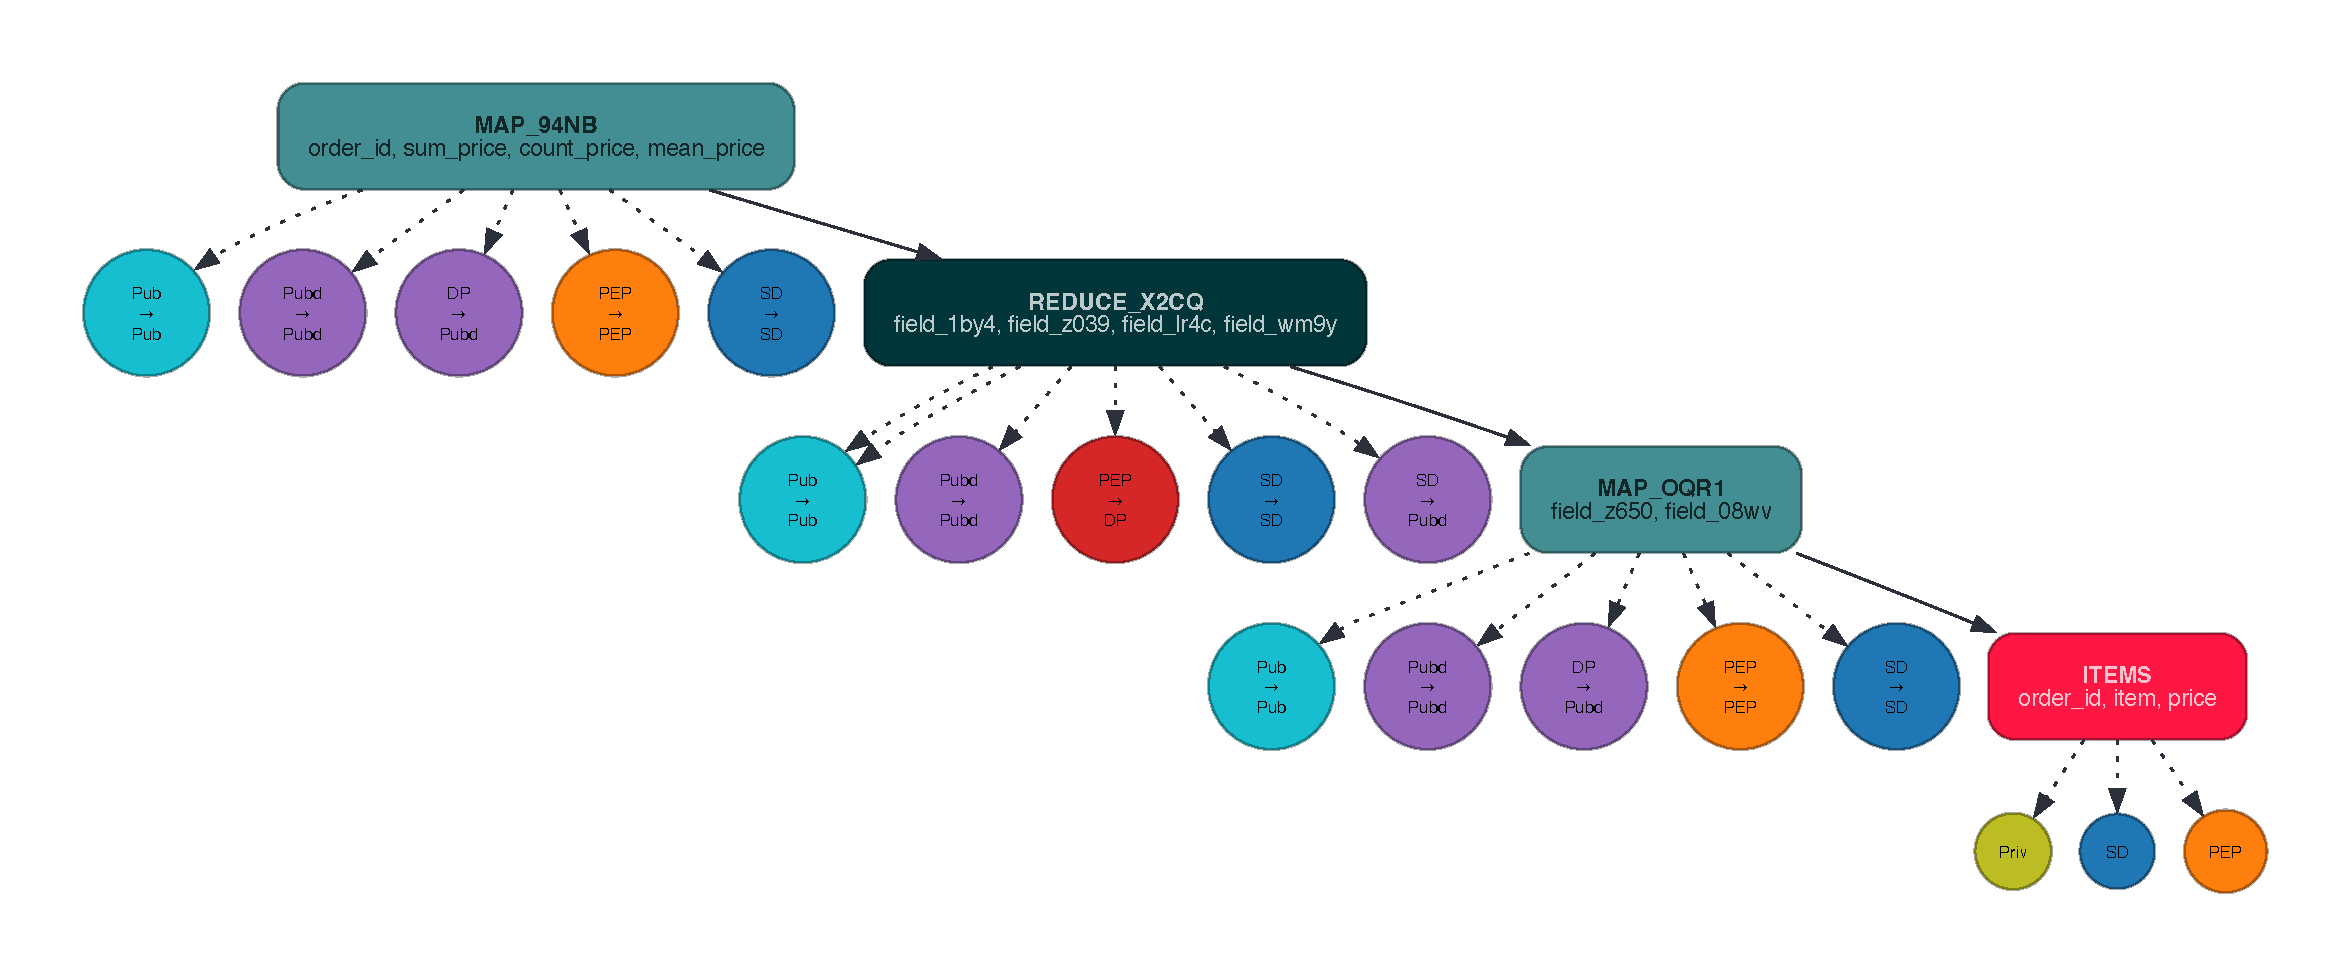
\includegraphics[width=1\linewidth]{figures/rewriting_rules_setting.pdf}
\caption{Rule Setting: Each node in the graph (rectangle) is assigned the applicable rules (circle) for that type of node. In blue, the *→SD rules, in orange the *→PEP type rules, in purple the *→Pubd rules, and in red the *→DP rules.}
\label{fig:rule_setting}
\end{figure}

\begin{figure}[!ht]
\centering
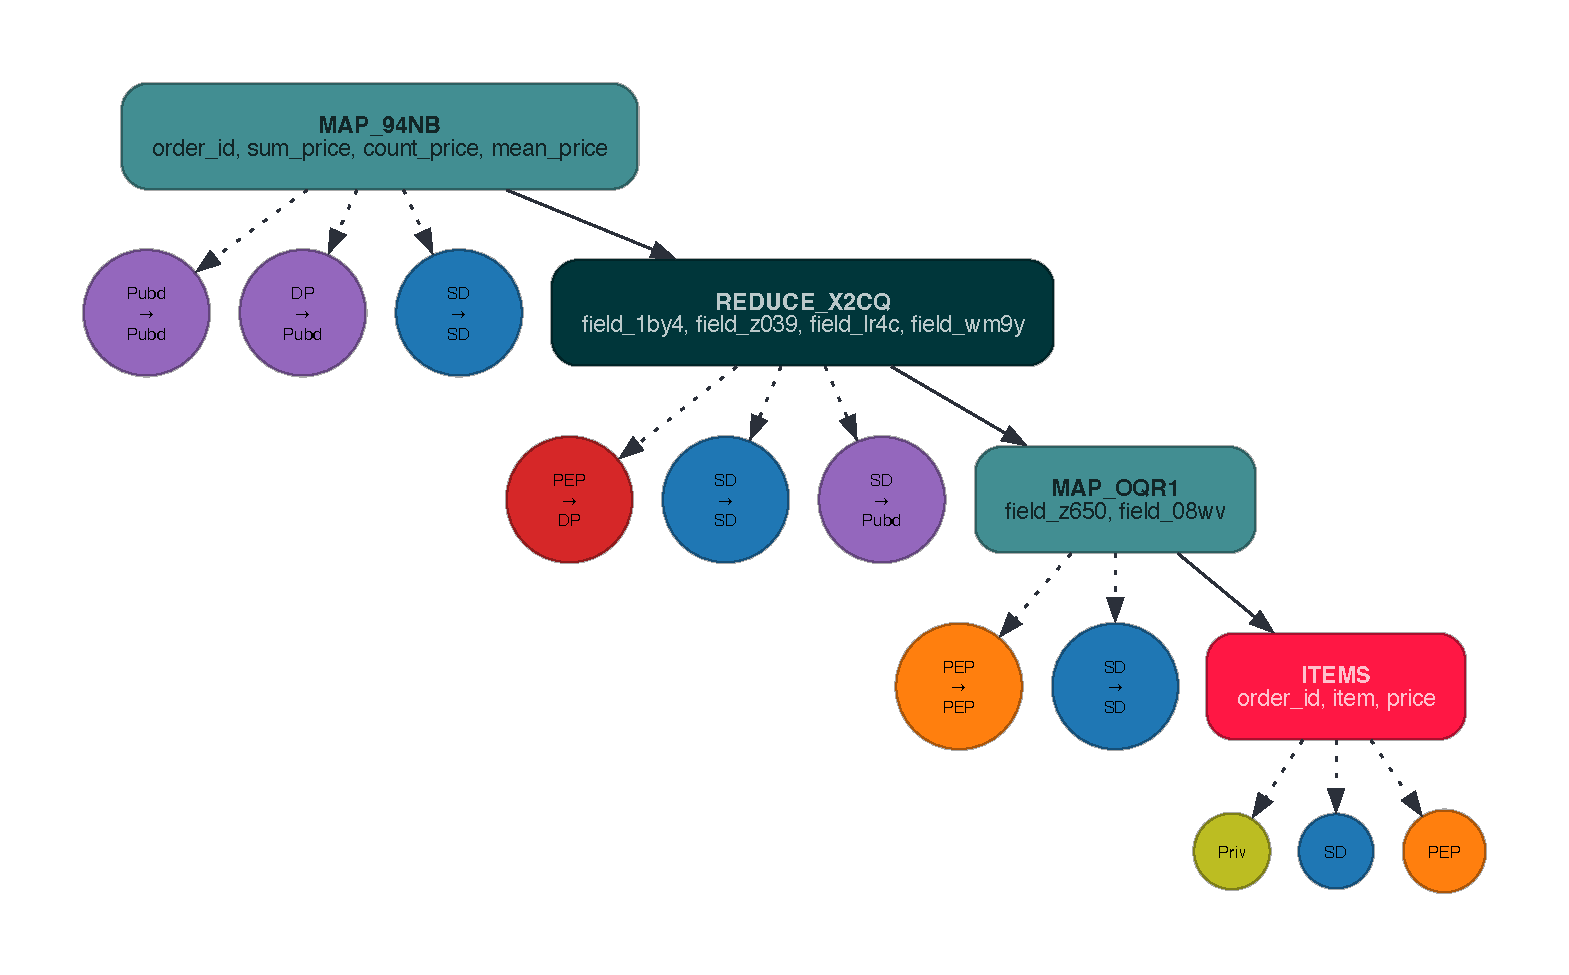
\includegraphics[width=1\linewidth]{figures/feasible_rewriting_rules.pdf}
\caption{Rule Elimination: Only feasible rules are retained.}
\label{fig:rule_elimination}
\end{figure}


\begin{figure}[!ht]
\centering
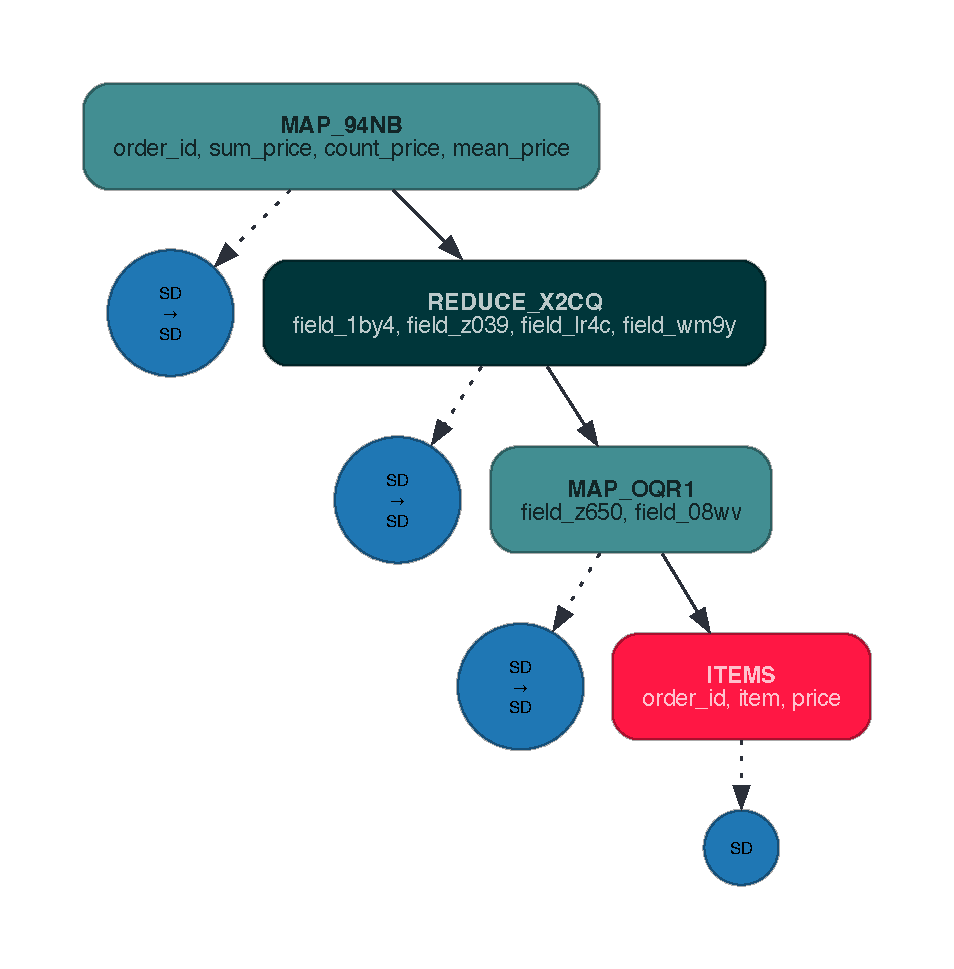
\includegraphics[width=1\linewidth]{figures/sd_allocation.pdf}
\caption{Example of SD Allocation: The sources of the graph are substituted with their synthetic equivalent.}
\label{fig:sd_allocation}
\end{figure}


\begin{figure}[!ht]
\centering
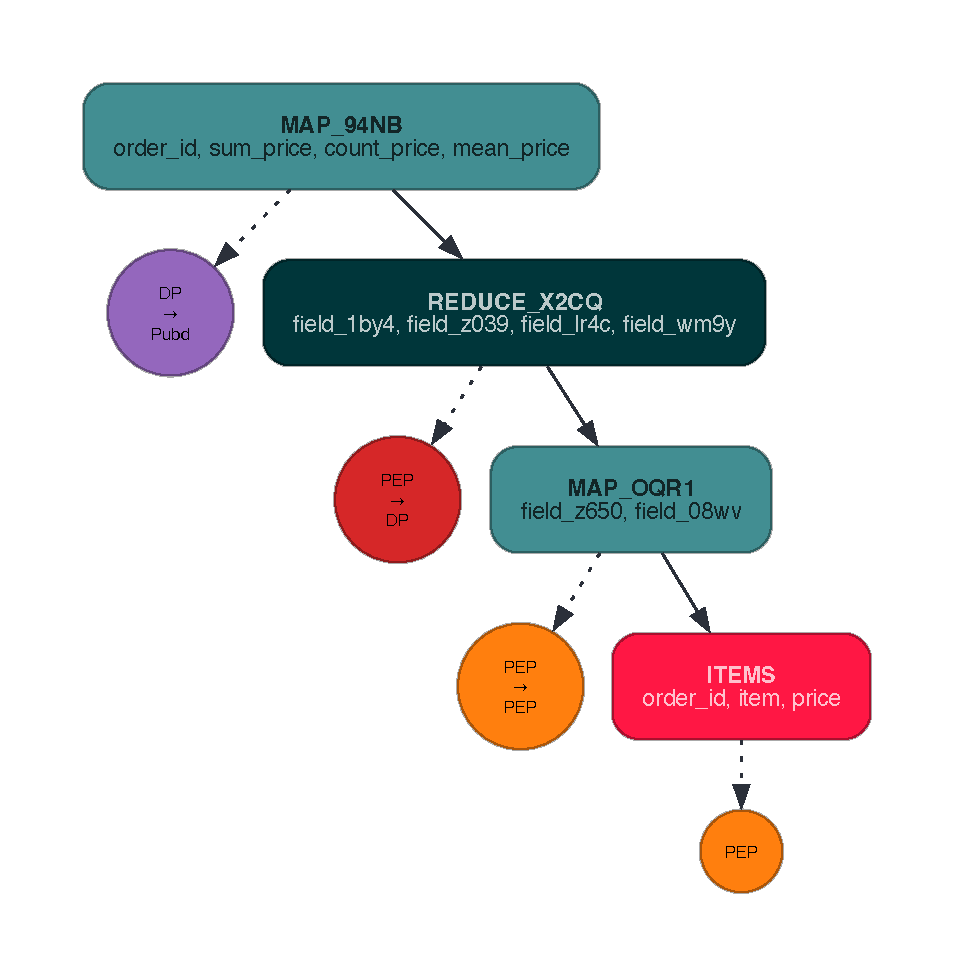
\includegraphics[width=1\linewidth]{figures/dp_allocation.pdf}
\caption{Example of DP Allocation: Rewrite in DP as soon as necessary (and possible).}
\label{fig:dp_allocation}
\end{figure}
